% !Mode:: "TeX:UTF-8"

\chapter{基于消息传播的人对间关系网络}
\label{ch:model}

本章将提出一个消息传播的人对间关系网络,简称PPRN。本章节将说明PPRN网络的特征提取模块、消息传播模块、消息池化模块,最后定义整个模型的优化方法和具体实现细节。


\section{基本框架}
首先,需要提到的是PPRN的输入和现有的模型是存在一些差别。对于\textbf{dual-glance}和\textbf{GRM}来说,输入是一张图片,两个人的包围盒坐标。在第一章的介绍中提到,本文的出发点是希望对人对间的关系进行建模。对于图像的社会关系理解任务,需要识别出图片上每个人对之间的社会关系,但是图像特征的模糊性和不确定性,这是一个很难的任务。利用上图上人对之间的关系信息,即结构信息,图像中人对间关系的结构信息能抑制对不准确检测结果。因此,PPRN网络的输入是以图片为单位而不是人对,每次同时输出一张图片上所有人对间的社会关系。PPRN主要是由3个模块组成,并且模型的主要预算模块是向量,以下提到的所有向量编码维度均为n维。如果将人之间的社会关系视作节点,本文对于图片上所有这样关系节点的全连接图成为\textbf{社会关系图谱},节点间的连边不含语义,采用类似于\textbf{GRM}的方式,利用特征提取模块得到的编码来初始化社交图谱上的关系节点。人对关系采用GRU来探索一个节点和图上其它节点间的交互,一张图片往往是一个场景,使用场景中其它节点的社会关系来对当前节点的社会关系消歧。此外,引入注意力机制对探索不同节点交互时的影响力。

如图\ref{fig:model-pprn}所示,PPRN模型是一个端到端的架构。PPRN模型接受一张图片和图片上所有人的包围盒的作为输入,经过前文提到的3个模块,并且每个模块的作用各有分工。模型首先提取图片中关于人和人对包围盒的特征,图\ref{fig:model-pprn}中的$p_{uij}$表示图上第i-th个人和第j-th个人的联合区域。$b_{i}$表示第i-th个人的包围和的坐标和包围盒的面积编码。在消息池化模块中,消息池化函数计算关系间的消息,然后作为下一轮GRU神经元的输入。其中$\oplus$表示一个可学习的权重参数。而对于消息传播模块,通过循环神经网络来实现通过反复传递消息来提醒当前节点目前场景中其它节点的行为,这个是图推理的一种实现方式,可以优化对社会关系的估计。在最后一次迭代时,利用GRU神经元最后的隐藏层的输出连接一个全连接层得到最后的预测结果。
\begin{figure}[htpb]
	\centering
	%	\includegraphics[width=0.48 \textwidth, trim=10 10 10 80,clip]{./pic/example_new.pdf}
	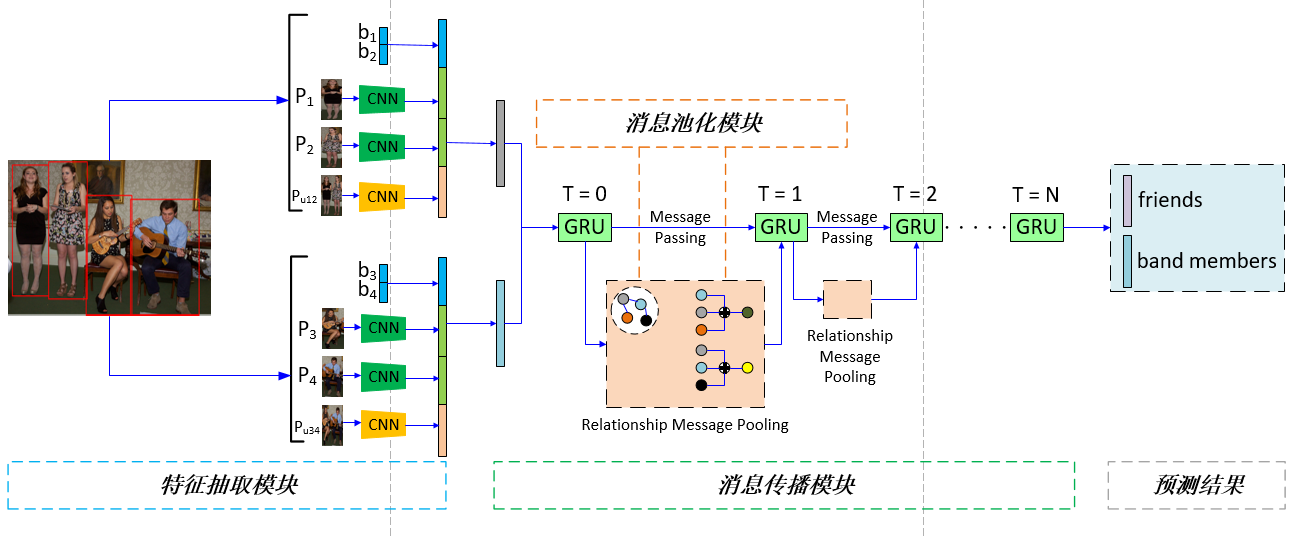
\includegraphics[width=0.98 \textwidth,clip]{model.png}
	%\hspace{0.02\textwidth}
	%\vspace*{-0.08cm}
    \caption{PPRN模型的结构示意图}
	\vspace*{-3.5mm}
	\label{fig:model-pprn}
\end{figure}

\subsection{特征抽取模块}


模型微调是指给定一个预训练模型,这里的预训练网络通常是在大规模标注数据集上训练好的模型,例如常用的预训练模型有Vgg和ResNet。此时的模型已经能很好的抽取大部分图片的信息,比如卷积神经网络的浅层往往是提取基础特征,例如边缘、轮廓等基础特征。深层卷积层提取抽象特征,例如脸型,而最后的全连接层根据特征组合进行连接分类。对于在大规模数据集上已经训练过的模型来说,已经具备了提取浅层特征和深层次抽象特征的能力。基于预训练的模型来新的数据集能节省很多的计算时间和计算资源,而且还能提升模型的效果。常见的模型微调方法是将我们现有的分类层替代预训练模型的最后一层,然后以较小的学习率微调前面的所有层,原因是不想过快的扭曲前面已经学习好的特征,然后着重训练最后的分类层。或者冻住预训练模型前面的若干层,微调后面的网络层。

特征提取模块包括物体的特征和人对的特征,对于人对的特征,采用的预训练模型是ResNet-101\cite{he2016deep},本文的做法微调模型的后2层和分类层。特征抽取模块的主要目标是提取出输入的图片和人的包围盒坐标区域的图像特征。因此,该模块首先修剪出三个小块,$p_1$ 和$p_2$ 为个体的区域,$p_{u}$ 为两个人区域的并集区域,这些区域的特征包含了用于识别关系的基本组成部分。这些区域首先被调整为大小224 $\times$ 224,然后输入三个ResNet,其中$p_1$ 和$p_2$ 的区域的网络是共享参数的。三个模型最后一个卷积层的输出拼接在一起,形成视觉特征向量$\mathbf{v}_1$。其次,位置信息同样很重要,对于其中的关系类别中的`` 无关系'',这单纯从视觉特征来判断是很难的,此时位置信息往往能起到很好的区分作用。我们表示一个包围盒$i$的特征为$b_i^{pos}$ = $\{ x_{i}^{min}, y_{i}^{min}, x_{i}^{max}, ~y_{i}^{max},~ area_{i} \}$ $\in$ $R^5$。 其中这些值都是相对位置。$x_{i}^{min}$和$y_{i}^{min}$是包围盒的左上角坐标,$x_{i}^{max}$和$y_{i}^{max}$是右下角坐标。最后这些特征拼接在一起后通过全连接层形成关系特征向量$\mathbf{v}_h$


\subsection{消息传递模块}

对于一张图片中$n$个人对的关系,通过特征抽取模块,得到了图片中所有人对关系的特征编码,$\{ v_{1},v_{2},...,v_{n} \}$,并且对于一张图片构成的社会关系图谱,是一张全连接图。对于特征抽取模块得到的关系向量编码通过如公式\ref{eq:model-hidden-init}所示,转换到一个低维空间,其中$ \varphi $可是视为全连接层。
\begin{equation} \label{eq:model-hidden-init}
    h_{i}^{0} = \varphi (v_{i})
\end{equation}

为了学习到图片中的场景信息信息对关系编码的约束,我们采用了循环神经网络来执行社会关系检测理解的推理工作。与Zheng\cite{zheng2015conditional}的模型不同的是,我们采用通用的RNN神经元来计算隐藏层状态。相比较LSTM,GRU少了一个门,因此更加简单并且参数较少,学习起来更快,因此本文采用的是GRU模块。我们采用第t步的隐藏层状态编码表示社会关系图谱中所有关系节点信息,关系节点的向量编码会随着RNN序列的长度每一步都更新。而关键的是每一步GRU的输入来自消息池化模块的输出,消息池化模块承担着关系节点间交互的任务。具体细节如公式\ref{eq:model-gru}所示,其中$\mathbf{v}_h$会当作GRU第一步的输入,并且此时的隐藏层的初始化为值为0的向量。这里的$\sigma$和$tanh$表示逻辑斯谛回归和双曲正切函数。$\bm{\odot}$操作表示点乘操作,$\gm{r}_t$表示重置门,$\bm{z}_t$表示更新门,下标$t$表示迭代步骤。$\mathbf{W}_r$和$\mathbf{W}_z$ 表示两个门需要的参数,这些参数可训练的。

\begin{equation} \label{eq:model-gru}
\begin{split}
\bm{r}_t &=  \sigma(\bm{W}_{r}[\bm{h}_{t-1}, \bm{x}_t]), \\
\bm{z}_t &=  \sigma(\bm{W}_{z}[\bm{h}_{t-1}, \bm{x}_t]), \\
\hat{\bm{h}_t} &= tanh(\bm{W}[\bm{r}_t \odot \bm{h}_{t-1}, \bm{x}_{t}])\\
\bm{h}_t &= (1 - \bm{z}_t) \odot \bm{h}_{t - 1} + \bm{z}_t \odot \hat{\bm{h}_t} \\
\end{split}
\end{equation}

\subsection{消息池化模块}

消息传递模块利用RNNs解决推理问题,但是在每个迭代步的时候,GRU单元会接受多个来自社会关系图上其他节点的消息,需要有一个聚合模块来将这些信息结合成一个有意义的编码向量。直观来看,常见的池化能实现这个功能,例如常用的最大池化和平均池化。在理解当前图片的社会关系图谱时,只利用上下文的结构信息中最相关的那部分是最合理的方式。而本文的消息池化模块也是出于这个目的提出的。下面将会说明简要说明注意力机制的基本情况。如公式\ref{eq:model-mp-atten}所示,其中第$t$步的节点$i$的前一步隐藏层状态为$h_{i,t-1}$,$m_{i,t}$表示来自其他节点消息的聚合,而$\bm{m}_{i,t}$将会作为第$t$步中公式
\ref{eq:model-gru}中输入,即$x_{t}$。其中符号[.]表示两个向量编码的拼接,$\sigma$表示激活函数,$\bm{w}$是需要学习的参数向量,$\bm{h}_{j \to i,t-1}$是节点j在第t-1步时的隐藏层编码,并且等同于
公式\ref{model-gru}中节点j的$h_{t-1}$

\begin{equation}
    \label{eq:model-mp-atten}
	\bm{m}_{i,t} = ~\sum_{j\neq i} \sigma{(~\bm{w}^T[~\bm{h}_{i,t-1},\bm{h}_{j \to i,t-1}~]) \bm{h}_{j \to i,t-1}}	
\end{equation}

%%%%%%%  注意力机制  %%%%%%%%%%%%


\subsection{物体信息微调模块}

%%%%%%%%%%%%%% 之后写  %%%%%%%%%%% 先空着
本文在模型\ref{fig:model-pprn}的基础上,本文实现了类似\textbf{dual-glance}的方法结合周边物体的信息,如图\ref{fig:model-atten}。当前模块主要包括两个步骤,利用faster-rcnn中的RPN(region proposal network)生成物体置信度高的区域,其次利用注意力机制得到关于周边物体区域的得分。

在一张图片中,往往会存在一些日常见到的物体,例如桌子、电脑、杯子,如果在一张图片中检测到了被杯子、桌子或者床等物体,那么当前的社会关系往往是``家庭''。因此本文在利用关系上下文的基础上,进一步加入周边物体信息来提升效果。但是在PISC和PIPA-relation数据集中,不包含物体包围盒的标注以及物体类别的标注,这里采用的方法是利用在大规模训练集上,例如COCO\cite{lin2014microsoft}预训练好faster-rcnn模型,利用其中的区域生成网络。区域生成网络的输入可以是任何大小的图片,输出是一些长方形的检测框,其中每个检测框都带有是否包含物体的得分。由于期望RPN和fast-rcnn共享有vgg\cite{simonyan2015very}(本文采用vgg,也可采用其他的预训练模型)生成的特征图,这里的vgg 网络有13个可训练的卷积层。
\begin{figure}[htpb]
	\centering
	%	\includegraphics[width=0.48 \textwidth, trim=10 10 10 80,clip]{./pic/example_new.pdf}
	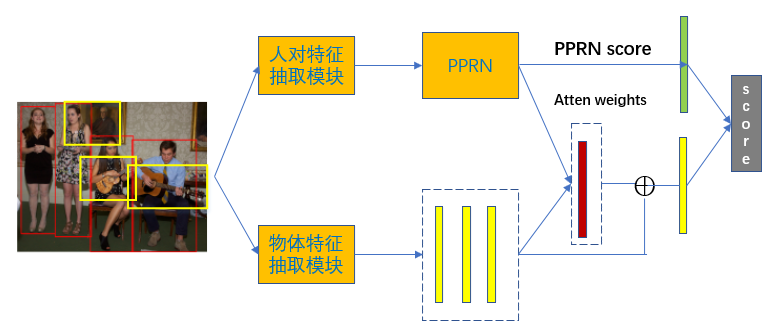
\includegraphics[width=0.98 \textwidth,clip]{model-atten.png}
	%\hspace{0.02\textwidth}
	%\vspace*{-0.08cm}
    \caption{PPRN模型的结构示意图}
	\vspace*{-3.5mm}
	\label{fig:model-atten}
\end{figure}

经典的方法生成检测框都非常耗费时间,例如RCNN和fasr-rcnn采用的选择性搜索,而faster-rcnn抛弃传统的方法,直接从特征图生成检测框,能极大的提升检测的速度。


\subsection{优化和实现细节}


